%%%% This Beamer example was created by LianTze Lim, April 2017.

%%%% This is a VERY simple and minimalistic beamer theme,
%%%% even reminiscent of marker pens on transparencies!
%%%% It mimics the look of the "seminar" package, which
%%%% can only be used with plain TeX.
%%%% There are also some comments and example to show how
%%%% to customise various elements, e.g. the font and colours.

\documentclass[12pt, aspectratio=169]{beamer}
%% If you'd like the default font size to be even larger, use 14pt or 17pt; these are supported by Beamer.

\usepackage[english]{babel}
\usepackage[utf8]{inputenc}
\usepackage[T1]{fontenc}
\usepackage{lmodern}
\usepackage[inkscapeformat=png]{svg}


%%%%%%%%%%%%%%%%%%%%%%%%%%%%%%%%%%%%%%%%%
% These lines should usually go into a .sty file,
% but I'll leave them here so that it's easier to
% see how to customise a Beamer theme.
% Remember, the Beamer manual is your friend!!
% http://texdoc.net/pkg/beamer
%
%% So if your re-definitions have a @ somewhere, you
%% _MUST_ put a \makeatletter before these lines and then
%% \makeatother after them. This trick can only be done
%% in the preamble! BUT if you're doing these re-definitions
%% in a .sty file (so that you \usepackage it later), you
%% don't need the \makeatletter and \makeatother.
\makeatletter

%% Set the left and right margins
\setbeamersize{text margin left=1em,text margin right=1em}

%% FONTS
\setbeamerfont{title}{series=\bfseries,size=\LARGE}
\setbeamerfont{subtitle}{series=\bfseries,size=\Large}
\setbeamerfont{frametitle}{series=\bfseries,size=\small}
\setbeamerfont{block title}{series=\bfseries,size=\normalsize}
\setbeamerfont{footline}{size=\normalsize}

%% COLOURS
%% If you'd like everything to have the same colour
%%\usebeamercolor{structure}
%%\setbeamercolor{normal text}{fg=structure.fg}

%% Add a line after the frametitle
\addtobeamertemplate{frametitle}{}{\vspace*{-1ex}\rule{\textwidth}{1pt}}

%% Use circular discs as itemized list markers;
%% there's an existing option in Beamer for it so I'll use it
\setbeamertemplate{itemize items}[circle]

%% Remove default navigation symbols (We'll add the ones we need in the footline
\setbeamertemplate{navigation symbols}{}


%% And before the footline... actually we'd like to re-define
%% the footline
%%\setbeamertemplate{footline}{%
   %% Beamer headlines and footlines are always full-paperwidth, so if you want the horizontal line to
   %% not span it entirely you'll need to do a bit of arithmetic
  %% \centering
   %%\begin{minipage}{\dimexpr\paperwidth-\beamer@leftmargin-\beamer@rightmargin\relax}
   %%\centering
   %%\rule{\linewidth}{1pt}\vskip2pt
   %%\usebeamerfont{footline}%
   %%\usebeamercolor{footline}%
   %% The frame number smack in the middle
   %%\hfill\insertpagenumber/\inserttotalframenumber
   %%\hfill%
   %% ONLY the navigation symbols we want at the far right.
   %% We use an \llap so that it takes up zero width, and doesn't throw the page number off-centre!
   %%\llap{\insertframenavigationsymbol\insertbackfindforwardnavigationsymbol}\par
   %%\end{minipage}\vskip2pt
%%}

\makeatother
%%%% END STYLE CUSTOMISATION %%%%%%%%%%%%



\title{X-ray Vision:}
\subtitle{A Different View of the Universe}
\author{Elisea Jackson}
%\institute{}
%%%\date{April 2017}

\begin{document}

\begin{frame}
  \titlepage
\end{frame}

% Uncomment these lines for an automatically generated outline.
%\begin{frame}{Outline}
%  \tableofcontents
%\end{frame}


\section{Some \LaTeX{} Examples}

\subsection{Static Night Sky}

\begin{frame}{Our Place in The Universe}
  
% Commands to include a figure:
\begin{figure}
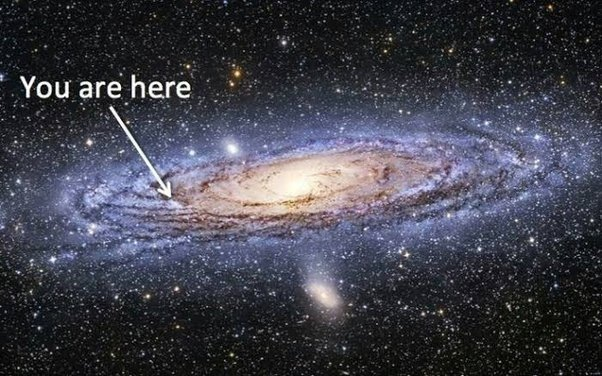
\includegraphics[width=0.7\textwidth]{we_here_gal_example.jpeg}
\end{figure}
\centering
Where Earth is located in the Milky Way Galaxy. 

%\begin{table}
%\centering
%\begin{tabular}{l|r}
%Item & Quantity \\\hline
%Widgets & 42 \\
%Gadgets & 13
%\end{tabular}
%\caption{\label{tab:widgets}An example table.}
%\end{table}

\end{frame}

\section{Some \LaTeX{} Examples}

\subsection{Figure}

\begin{frame}{Our View of The Universe}
  
% Commands to include a figure:
\begin{figure}
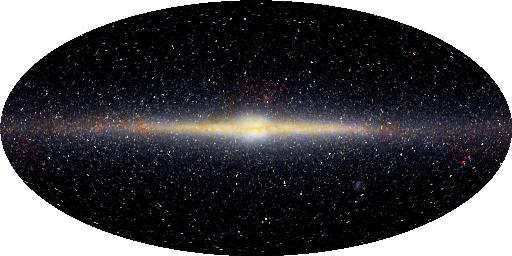
\includegraphics[width=0.7\textwidth]{Optical_light.jpg}
\end{figure}
\centering
View of the Galaxy using the Galactic Coordinate System.
\end{frame}

\subsection{Figure}
\begin{frame}{What if we could see X-rays?}
  
 \begin{itemize}
  \item Steady X-Ray Stars
  \item X-Ray Bursters
  \item X-Ray Pulsars
  \item Soft Gamma Repeaters
 \end{itemize}
\end{frame}

%possible place to show my Model

\subsection{Neutron Stars}

\begin{frame}{Neutron Stars}
  
  \begin{block}{Formation}
    Are formed through a supernova, when a giant star collapses in on itself. They are about 12 miles in diameter.
    %larger stars form black holes while smaller stars form a nuetron stars.
  \end{block}

  \begin{block}{Magnatars}
    \begin{itemize}
    \item Magnetic field of $10^{13}$ - $10^{15}$ gauss.
    \item Rotaional period is about 2 - 10 seconds.
    \end{itemize}
  \end{block}

  \begin{block}{Pulsars}
    \begin{itemize}
    \item Rotational period ranging from milliseconds to seconds. 
    \end{itemize}
  \end{block}

\end{frame}

\begin{frame}
  
% Commands to include a figure:
\begin{figure}
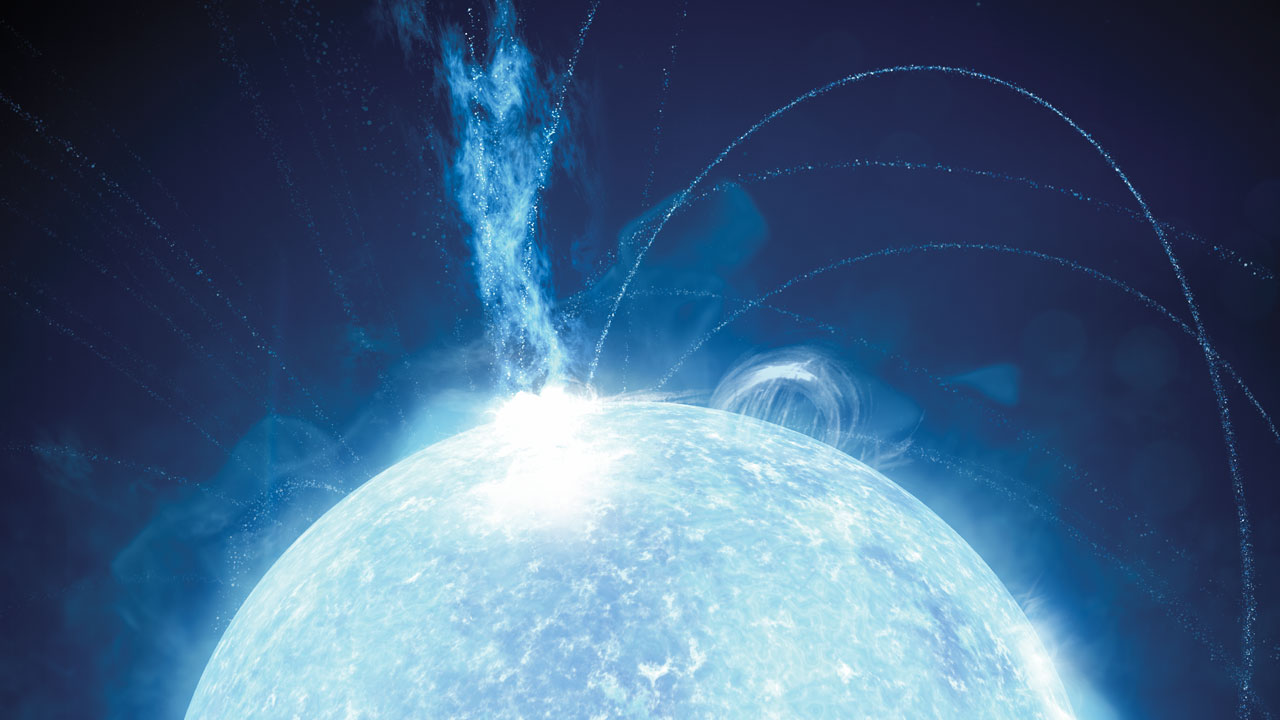
\includegraphics[width=\textwidth]{softrepeater.jpg}
\end{figure}

\end{frame}

\begin{frame}{Soft Gamma Repeaters}
  
% Commands to include a figure:
\begin{columns}
          \column{0.5\linewidth}
             \centering
               \begin{figure}
                 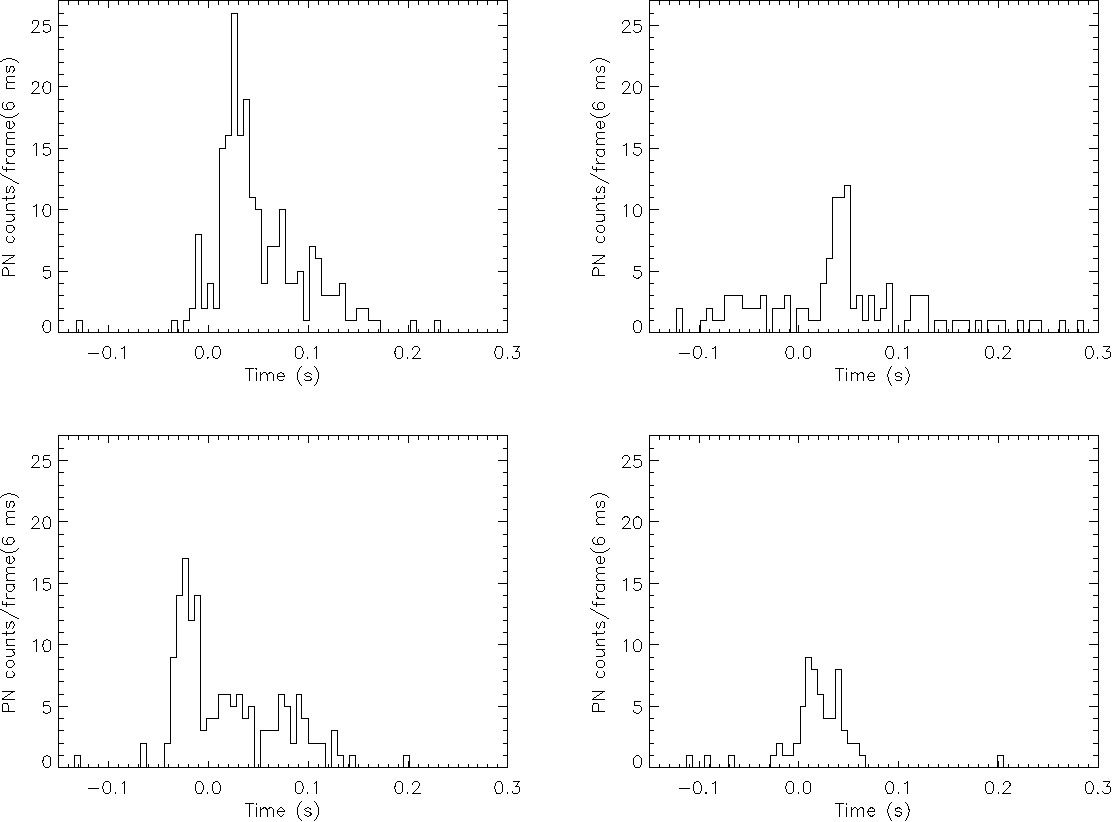
\includegraphics[width=\textwidth]{Sgr1806-20.png}
               \end{figure}

           \column{0.5\linewidth}
             \begin{itemize}
             \item Occur on Magneters
             \item Caused by Starquakes
             \item The rapid spining of star causes pulsation.
             \end{itemize}
            
         \end{columns} 
\end{frame}

\begin{frame}{Soft Gamma Repeaters}
  \centering
  \begin{figure}
    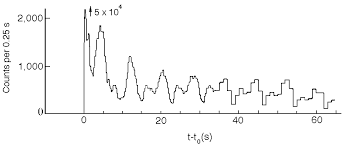
\includegraphics[width=0.75\textwidth]{big_sgr.png}
  \end{figure}
  Flare observed March 5th, 1979.
            
\end{frame}


\begin{frame}
  
% Commands to include a figure:
\begin{figure}
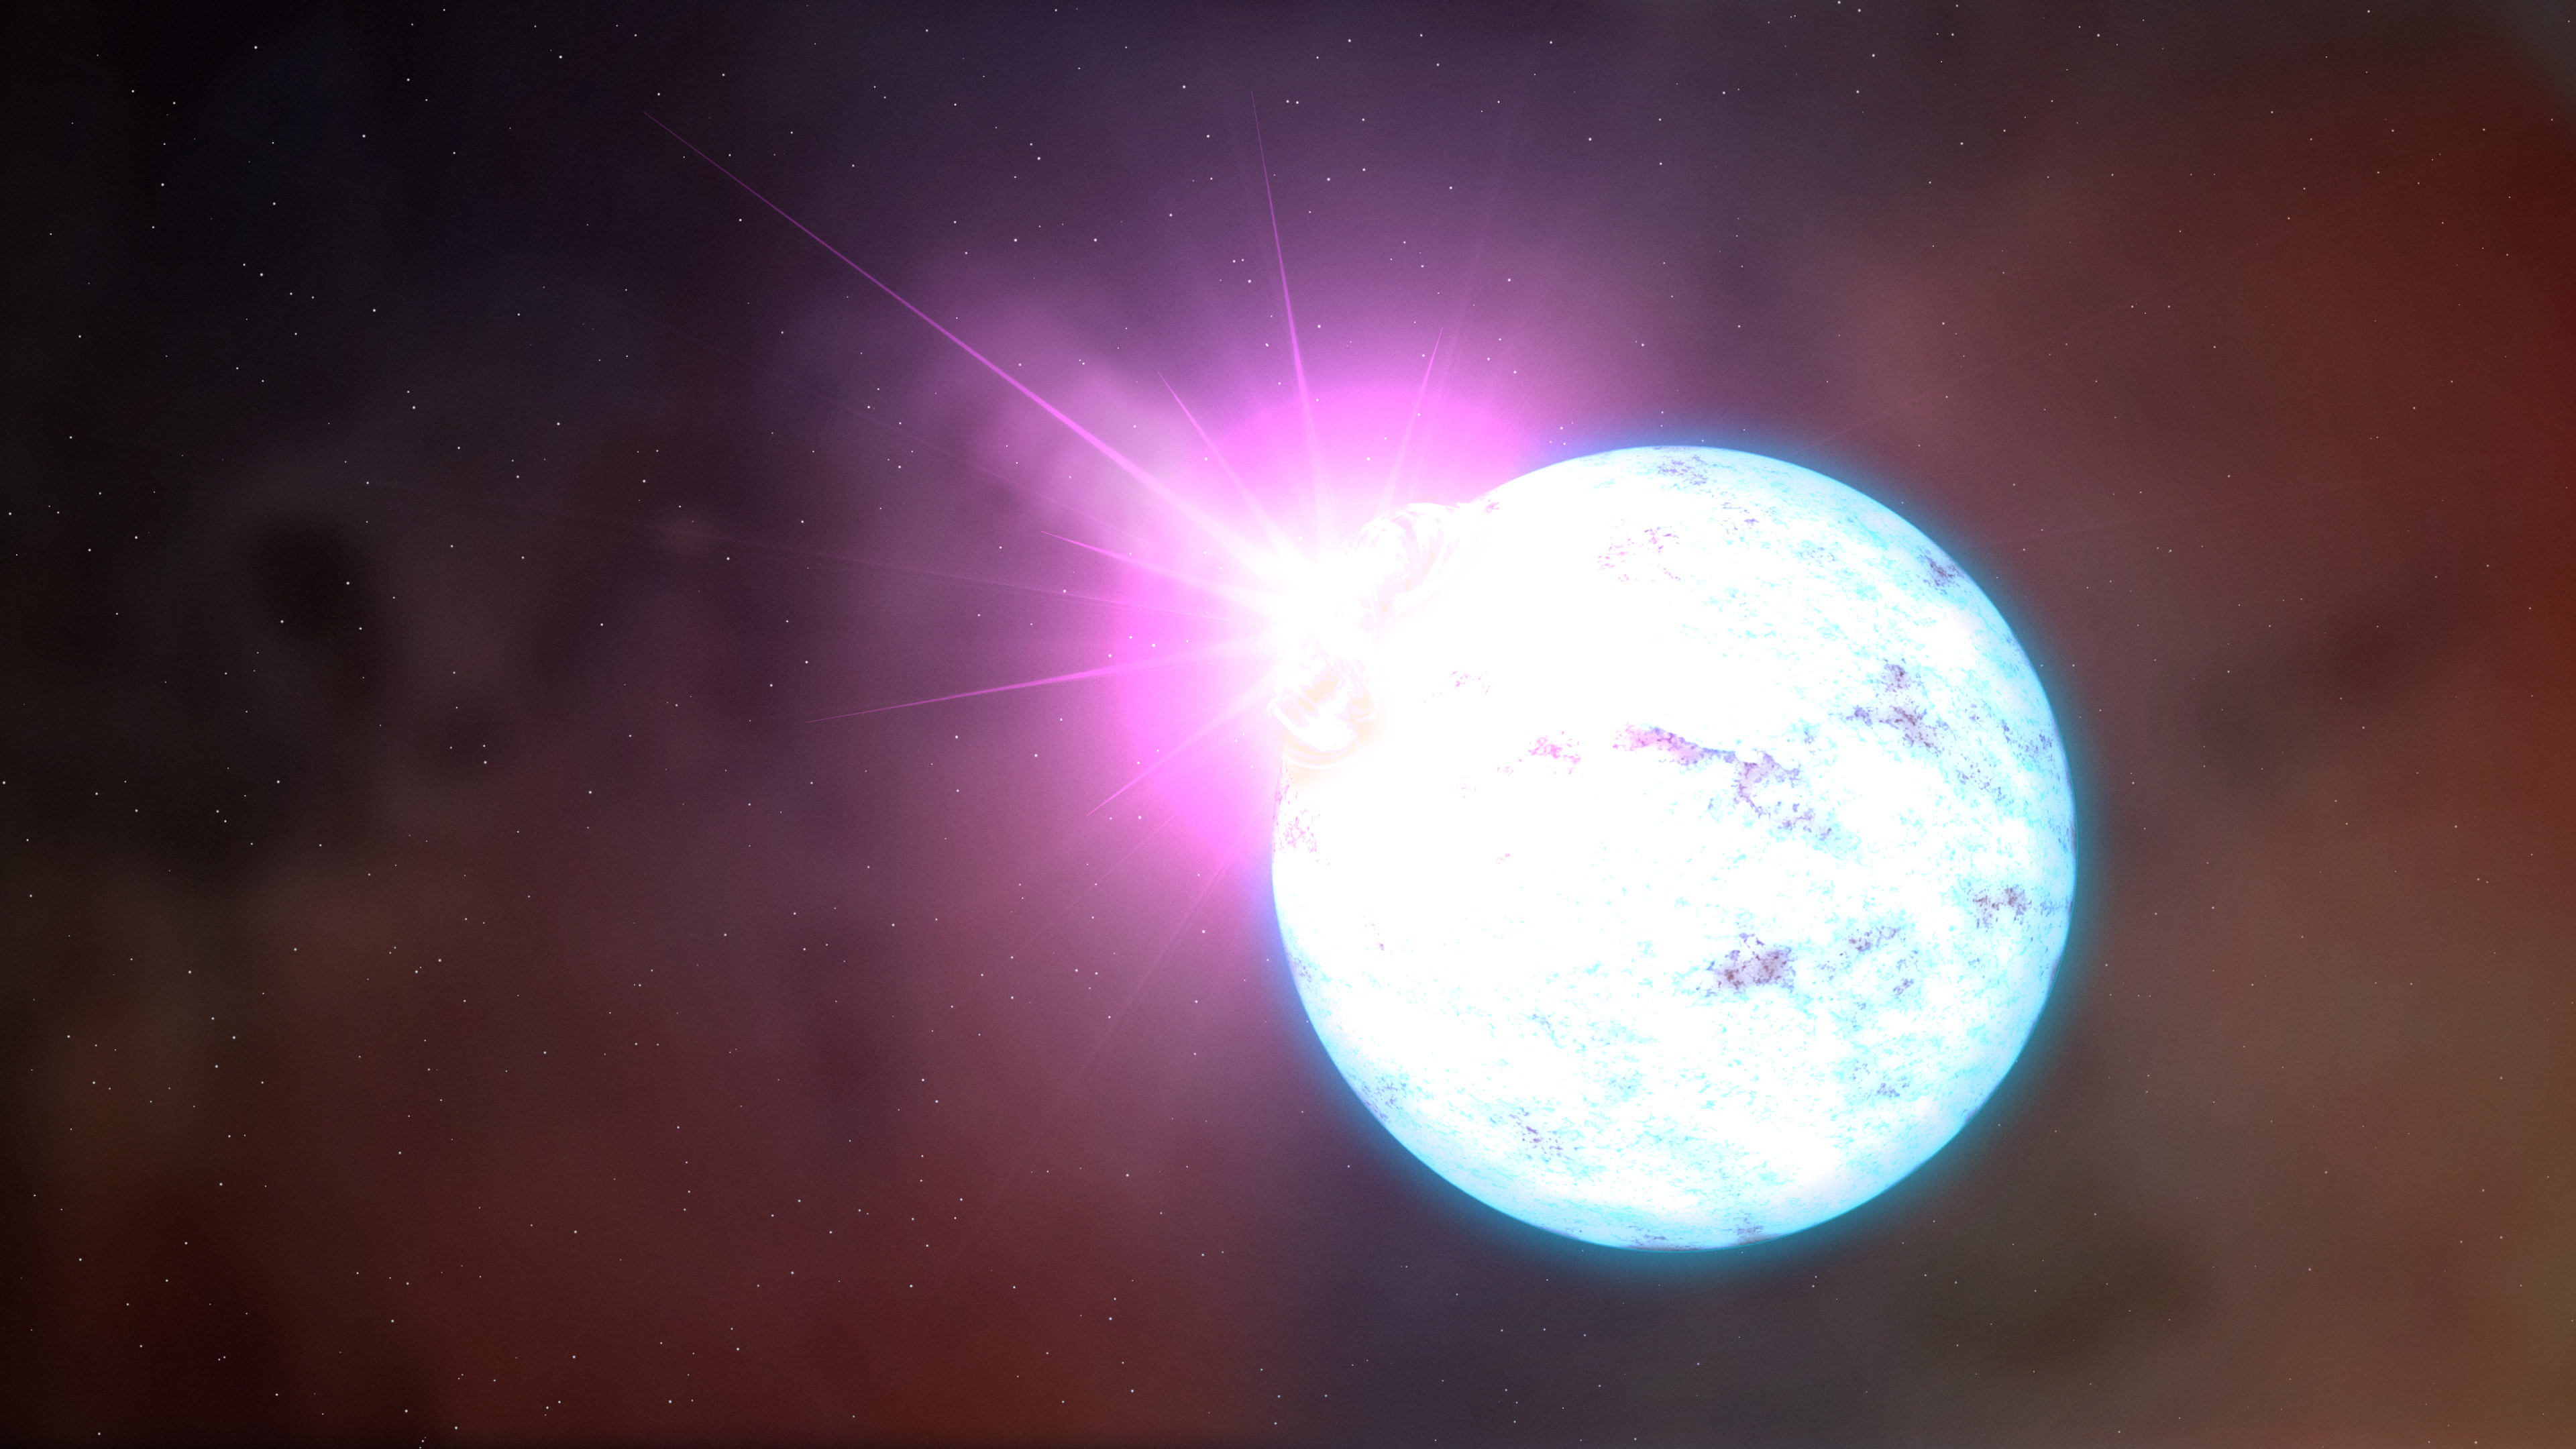
\includegraphics[width=\textwidth]{SGRart.jpg}
\end{figure}

\end{frame}


\begin{frame}{X-Ray Pulsars}
  
% Commands to include a figure:
\begin{columns}
          \column{0.32\linewidth}
             \centering
               \begin{figure}
                 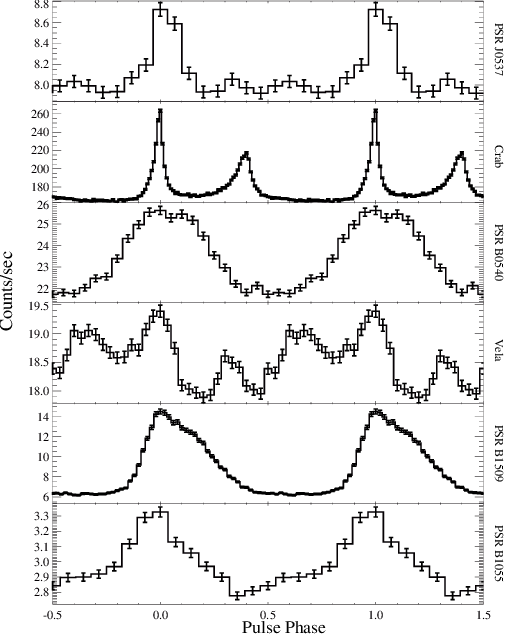
\includegraphics[width=\textwidth]{pulsars.png}
               \end{figure}

           \column{0.58\linewidth}
           %Good place to talk about how SGR where confused with GRB for long time. 
           Pulsar profiles can all look very different from each other. The charts on the right show XMM-Newton pulse profiles of the different pulsars. From top to bottom the pulsars have periods ranging from 16ms to 197ms.
           %with periods of 16 ms, 33 ms, 51 ms, 89 ms, 151 ms and 197 ms, respectively. The energy band in all cases is 0.2–12 keV.  

         \end{columns} 

\end{frame}


\begin{frame}{Crab Nebula}
  
% Commands to include a figure:

\begin{figure}
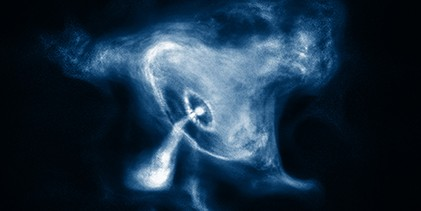
\includegraphics[width=0.8\textwidth]{crab_xray.jpg}
\end{figure}
\centering
The Crab Nebula Observed in X-rays

\end{frame}


%\vskip 1cm

%\begin{block}{}
%\end{block}



\section{Some \LaTeX{} Examples}

\subsection{Figure}

\section{Some \LaTeX{} Examples}


\begin{frame}{X-Ray Bursters}
  
% Commands to include a figure:
\begin{columns}
          \column{0.34\linewidth}
             \centering
               \begin{figure}
                 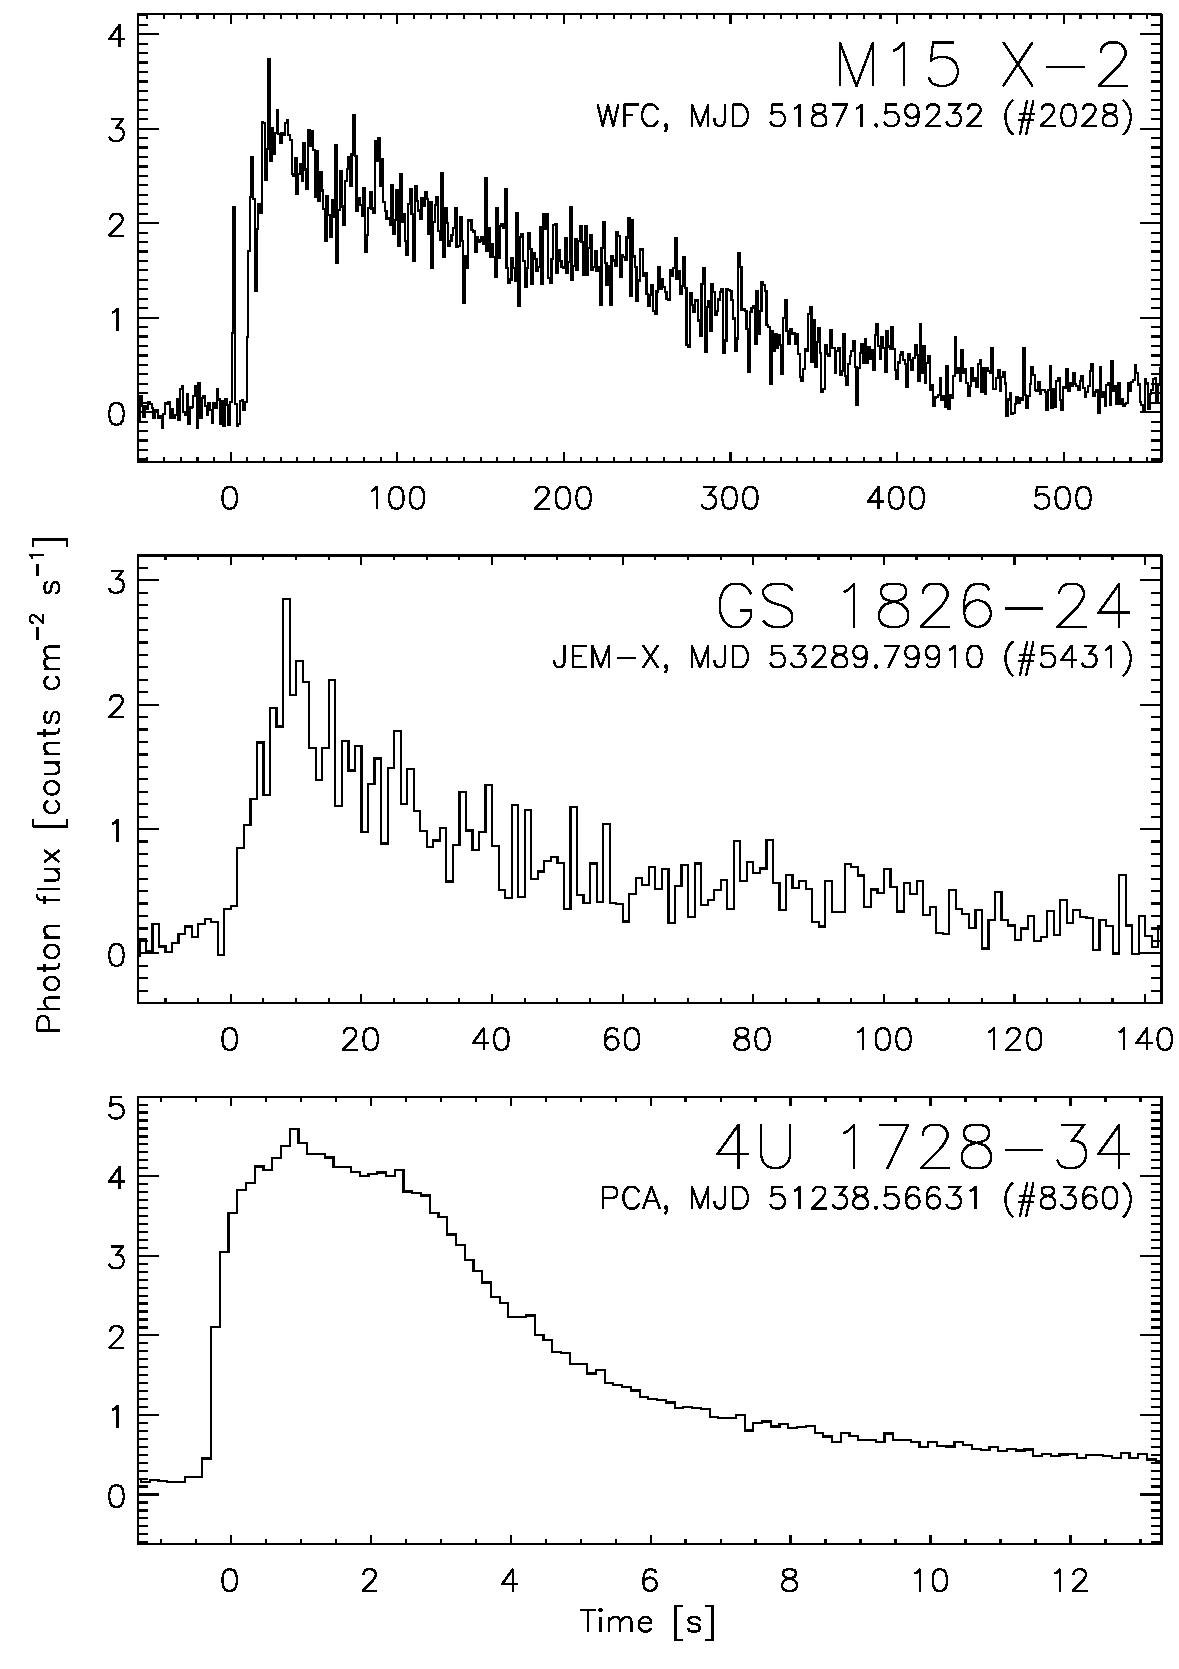
\includegraphics[width=\textwidth]{graph_burster.jpg}
               \end{figure}

           \column{0.58\linewidth}
              X-Ray bursts are caused by the accretion of matter on the surface of the Neutron Star. The figure on the left shows time profiles of typical X-ray bursters.
         \end{columns} 

\end{frame}

\begin{frame}{X-Ray Bursters}
  
% Commands to include a figure:

\begin{figure}
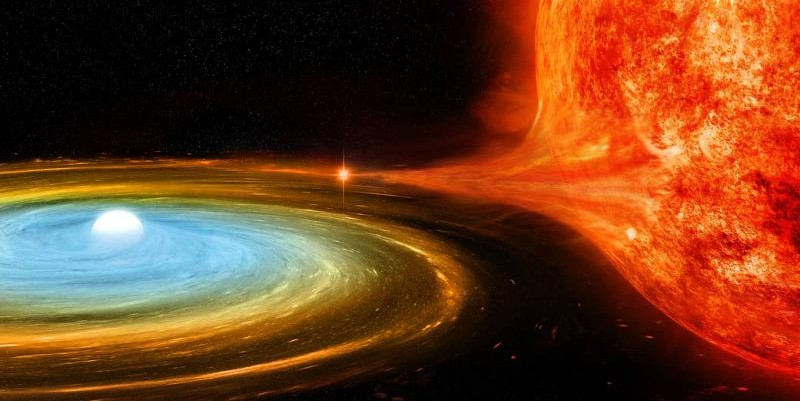
\includegraphics[width=\textwidth]{Xburster2.jpg}
\caption{\label{fig:your-figure}Caption goes here.}
\end{figure}

\end{frame}


\subsection{Mathematics}

\begin{frame}{Monte Carlo}

\begin{columns}
  \column{0.4\linewidth}
    \centering
      \begin{figure}
        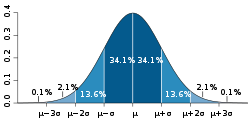
\includegraphics[width=\textwidth]{probability.png}
      \end{figure}
      \column{0.5\linewidth}
   Monte Carlo modeling allows for us to model various results when there are random variable involved. 
 
\end{columns}
\end{frame}

\begin{frame}{Monte Carlo}
Let $\sigma$ equal the standard deviation while $\mu$ determine the mean. 

Depending on $\mu$ and $\sigma$ we can create different distributions. 
\begin{columns}
  \column{0.5\linewidth}
    \centering
      \begin{figure}
        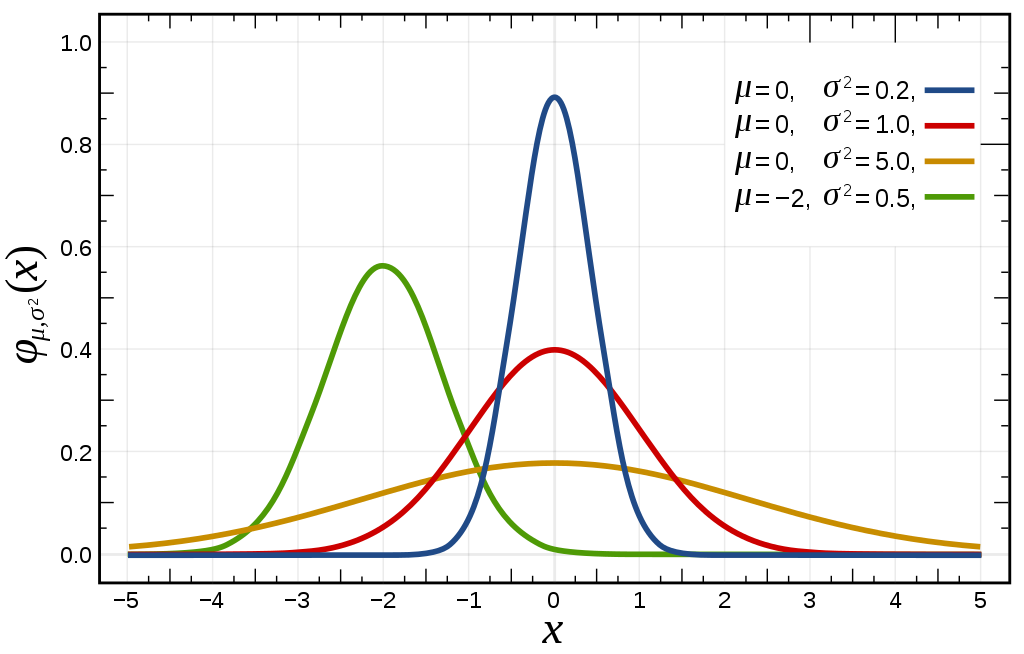
\includegraphics[width=\textwidth]{1024px-norm.png}
      \end{figure}
      Probability Density Function
   \column{0.5\linewidth}
     \centering
       \begin{figure}
         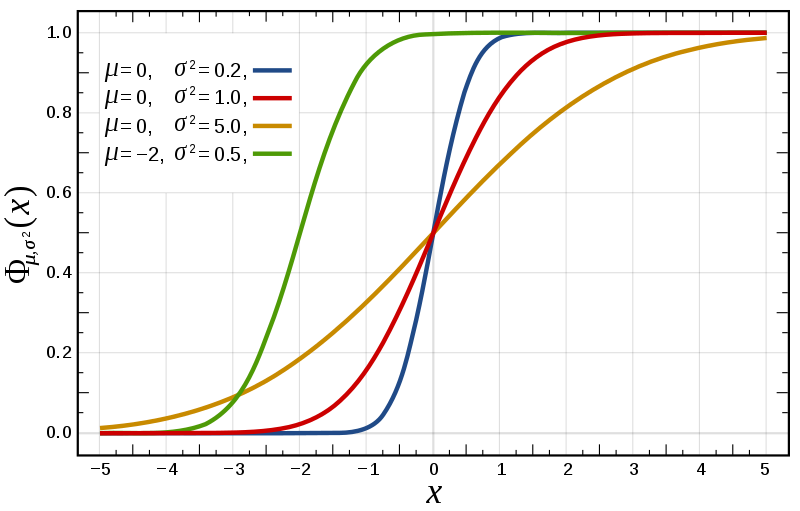
\includegraphics[width=\textwidth]{800px-dist.png}
       \end{figure}
       Cumulative Distribution Function
\end{columns}

\end{frame}

\begin{frame}{Inverse Error Function}
  \begin{figure}
       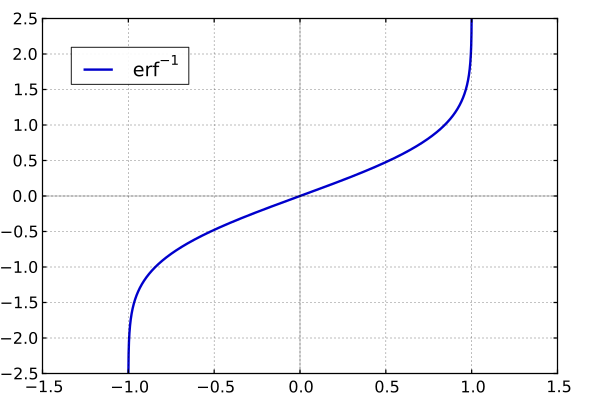
\includegraphics[width=0.5\textwidth]{erf_inv.svg.png}
  \end{figure}
  \centering
  The inverse error function allows for generating a random number with a probability distribution. 
\end{frame}

\subsection{Mathematics}


\begin{frame}{Summary}
  \begin{columns}
    \column{0.5\linewidth}
    \centering
    \begin{figure}
      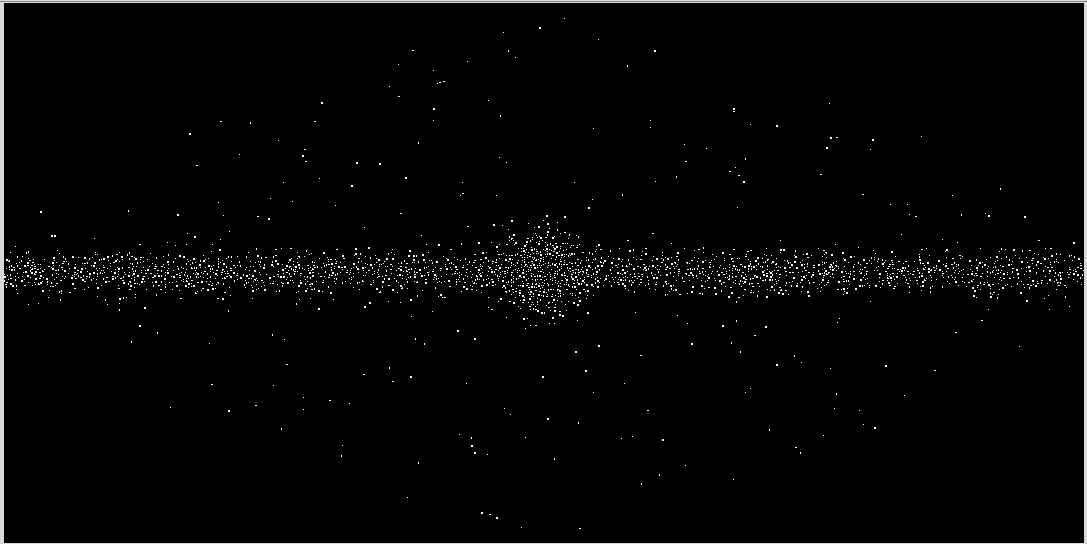
\includegraphics[width=\textwidth]{static.png}
    \end{figure}
    Model of the optical sky.
    \column{0.5\linewidth}
    \centering
    \begin{figure}
      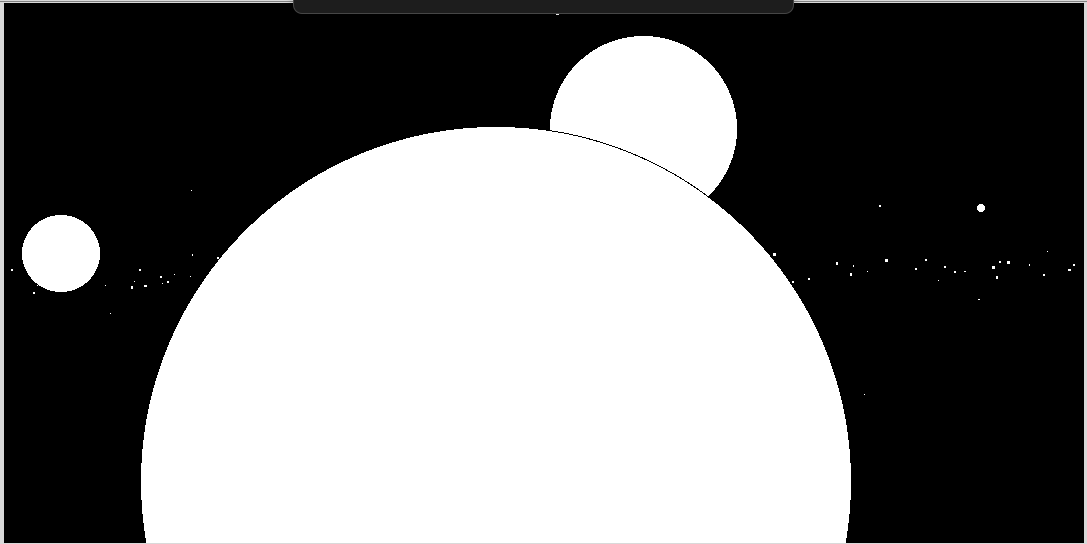
\includegraphics[width=\textwidth]{dynamic.png}
    \end{figure}
    Model of X-ray sky
  \end{columns}
\end{frame}

\begin{frame}
  \begin{figure}
       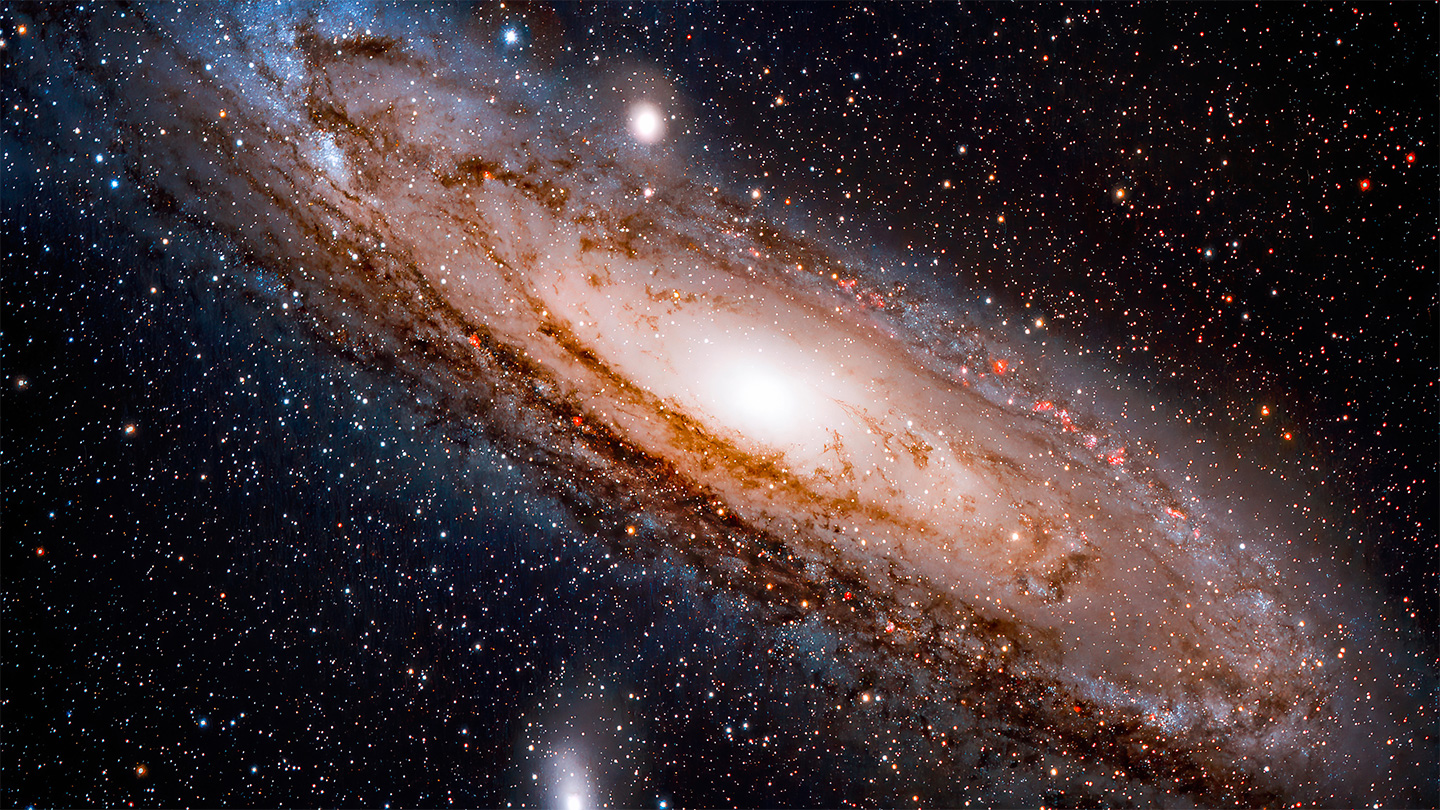
\includegraphics[width=\textwidth]{end_milkyway.jpg}
  \end{figure}
\end{frame}
  
%\begin{frame}{Refrences}
 % list refrences
%\end{frame}

%\begin{frame}{Refrences}
 % list of refrences continued
%\end{frame}

\end{document}

%Look for oprotunity to tell GRB SGR deiscovery starting with the treaty to not use neuclear weapons in space. 
